\documentclass{article}
\usepackage{fullpage,mathtools,amsfonts,graphics}
\author{Tucker DiNapoli}
\title{Numerical Analysis of the Korteweg de Vires equation}

\begin{document}
\maketitle
\section{Introduction}
A solver for the one dimensional Korteweg-de-Viers equation was written using C
and parallized using openmpi. The resultant data was plotted with gnuplot in
order to visualize the results. On inspection the plots are consistant with
results for the methods and initial conditions used. The algorithms used are
embarssingly parallel and so parallisation was trivial, and resulted in a
noticable speed up in the code.
\section{KdV Equation}
The Korteweg-de-Vires is a one dimensional partial differential
equation, of the form \[\partial_tu+\partial_x^3u-6u\partial_xu=0\]
The equation is primarily used to model waves in shallow water, and other
similar phenomena. The equation can be analytically solved via the
inverse scattering transform, or one of several numerical methods. The
stable solutions of the KdV equation take the form of solitons, waves
that move with a fixed shape.
\subsection{Initial Conditions}
In order to solve the KdV equation one must start with some sort of
initial condition defining the state of the system. In this case the
initial condition used was \[u(x)=-12\cdot csch(x)^2)\] the values of
x used were x from \(x=-1.5\pi\) to \(x=1.5\pi\) by steps of
\(\pi/32\).

\section{Numerical Analysis}
The techniques used in solving this problem were numerical differentiation
using a 5 point finite difference scheme and Runga-Kutta forth order(rk4) time
stepping. The KdV equation requires the first and third derivatives of u with
respect to x these are calculated using the 5 point finite difference formula
\[\frac{\mathrm{d} u_n}{\mathrm{d}
x}=\frac{C_1u_{n-2}+C_2u_{n-1}+C_3u_n+C_4u_{n+1}+C_5u_{n+2}}{C_6\Delta
x^{C_7}}\] in this equation \(C_1-C_7\) constants dependent on the order of the
derivative and \(\delta x\) is the x distance between \(u_n\) \&
\(u_{n+1}\). %put in actual coefficients?  Looking at the KdV equation, once the
derivatives of u have been found the time step of u can be calculated via the
equation \[\partial_tu=-\partial_x^3u+6u\partial_xu\] by using rk4 time
steping.%maybe more?

\section{Code}
\subsection{Code structure}
There are several pieces of source code that were written for this
project. Initally code was written in a generic way, the code for the rk4
algorithm was written using function pointers, as was much of the code for the
kdv implementation. The reason for this was to let the program be extensible,
so for example different in initial conditions could be used. This code was
difficult to work with, as it resulted in a large number of variable parameters
and function pointers. This code can be found int the kdv.h,kdv.c,main.c and
calculus.c and h files. An attempt was made to simplify this code using a
structure called udis(for u-discreet) to consolidate much of the variable
parts of the code into one manageable block. This also proved to be too
difficult to work with. This code can be seen all files with udis in the
name. Eventually an attempt was made to write a simple and limited, but working
version of the code. This code is located in the kdv-simple.c file, with some
code from calculus.c used. This code uses specifics of the kdv equation to
simplify much of the code, the rk4 algorithm does not have a time dependent
part, and works on full arrays and all function pointers were removed from the
code.
\subsection{Parallelization}
An attempt was made to insure all functions were pure, that is the
functions do not modify their arguments. This is the approach used in many
functional programming languages such as lisp,haskell,ml,etc. The advantage of
this technique is that it makes paralleling the code trivial, for example the
function u\_discrete which calculates \(-\partial_x^3u+6u\partial_xu\) can be
run in a parallel for loop as the original array is not modified. While in this
particular program there was not a huge benefit from this in more complicated
programs the benefits of functional programming techniques can be significant
as it eliminates much of the trouble with parallel programming, which is
coordinating access to mutable data between threads.
\subsection{Data Manipulation}
Initially the program wrote the data at every time step to a file, this
significantly increased the runtime of the program and made working with the
data near impossible. So the code now writes the data to file at a
predetermined interval which should be set based on the size of the time
interval. The data is written to a file named {Number}.txt where number is the
number of time steps so far padded with leading 0's if necessary to reach 6
digits. This data is stored in a directory called kdv-data. The data is
visualized using gnuplot, the shell script gnuplot.sh generates a gnuplot
script plot.gpi using the current files in kdv-data(and so must be re-run if
the data is changed). The file plot.gpi is a script that will generate an
animated gif called animate.gif that shows the progression of u through time.
The gnuplot.sh script can be modified(via commenting/uncommenting lines) to
generate a single .png image containing a superposition of all of the data.
\section{Data}
Unfortunately despite the best efforts of the author, the data generated does
not match the expected values. What is expected is a soliton solution,
consisting of a single pulse moving from left to right. As can be see in the
example plot below this is not at all like the data that was generated.
\begin{figure}
  \centering
  \caption{KdV data}
  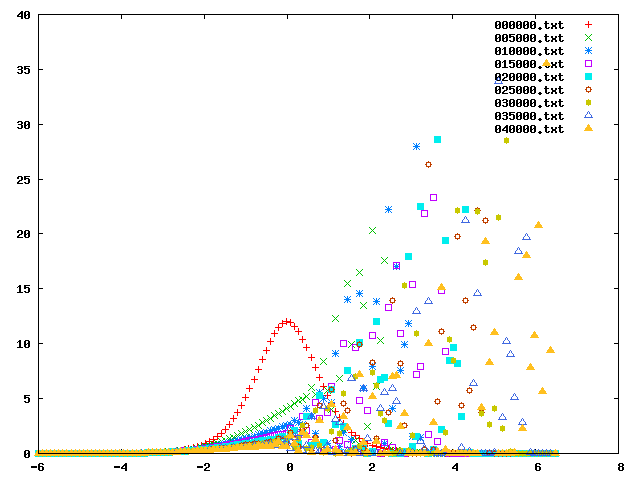
\includegraphics[scale=0.5]{data}
\end{figure}
\subsection{Error Analysis}
It is likely that the cause of this error is a small programming error. The
author believes the basic algorithms used to have been programmed correctly and
reasonable values used for the initial conditions and the space and time
steps. Because the data is generated via iteration a small error (for example
the addition/omission of a minus sign or accidental shifting of array indices)
could cause the results to be completely different than the expected values.
\section{Conclusion}
While the actual result of this project was not achieved much of the
work done was solid and the knowledge gained through this project will
be useful in the future. A simple analysis of the development process
and its errors would be that the code was developed using bottom up
programming which ultimately did not fit the programming language
being used. A much more in-depth analysis is included as an
appendix. A key lesson learned from this project is to start with
writing specific code (in this case code specific to the kdv equation)
and then after that code works to generalize to different problems (in
this case other 1-D partial differential equations).
\pagebreak
\section{Appendix:Analysis of Development}
Ultimately the development process for this project was flawed considering the
programming language used. The way in which the author writes code is conducive
to the use of a bottom up style of development. This style of development is
best done using a functional style, with incremental testing using a read eval
print loop(repl). The repl used in development was cling a c++ interpreter
developed by cern for use in the root programing environment. Cling is likely
the most sophisticated c/c++ currently available, it is based off llvm and its
c compilier clang and can run almost all c code in an interactive environment
(the interpreter is for c++ but as c++ is a near superset of c, c code runs
fine). The issue with this development technique for c code comes not from a
lack of an interpreter as one might think but from the language itself. As
functions in c are a sort of second class object(they can't be created at
runtime but can be passed as arguements via function pointers) traditional
functional programming techniques are difficult in c. The biggest difficulty in
using bottom up programming in c is that incremental testing is very difficult
for several reasons, for example the fact that c code will not
compile if references functions or datatypes that have not been declared yet,
this forces functions and datatypes to be determined first, and losing the
fluidity and flexibility of bottonm up programming. A final note on the use of
c is that of macros, coming from lisp c macros are very dangerous, in lisp
macros are a fundamental, flexible and ultimately safe part of the language
that allow code to be generated dynamically. C macros are ultimately just text
substitution, the c pre-processor does not understand c and so macros are not
subject to the rules of c which can easily lead to broken code. Without macros
bottom up programming is difficult, and somewhat more inefficient, yet using c
macros comes with a set of issues that make their use prohibitive.

There are several solutions to these issues to be considered in considered in
development of future high performance programs. There are two obvious
solutions, either do not use C or do not use functional programming. The latter
of these is not a likely solution as it violates the way in which the author
thinks of programs. The former however is viable, while traditionally functional
programming languages have been seen as slow advancement in compiler technology
and programming techniques have rendered this untrue. Good performance can be
obtained with a number of functional programming languages, but only one can
achieve performance equal or better that c, that language is ats. ATS uses
theorem proving to prove the safety of things like array bounds, pointer
arithmetic, buffer overflows and division by zero at compile time, this allows
the compiled program to achieve speeds equal to equivalent c code. Another
benefit of ATS is that it pushes error checking to compile time forcing
incremental testing. Using ATS is the best solution as it allows functional
programming with no speed penalty, however if for some reason this is not a
viable option better use of cling and safe use of the c pre-processor could be
used to mitigate some of the challenges faced during programming in this
project
\end{document}
